\Chapter{Die ASCII-Unit}

\label{ch:asciiunit}
Die ASCII-Unit ist f\"ur die Textausgabe auf dem Monitor zust\"andig.

\begin{figure}[!htbp]
	\centering
	\label{fig:exampletext}
	\includegraphics[width=0.7\textwidth]{asciiunitexample.png}
	\caption[Beispiel f\"ur die Textausgabe]{Beispiel f\"ur die Textausgabe: jedes darstellbare Zeichen wird abgebildet}
\end{figure}

\Section{\"Uberblick}

Die ASCII-Unit gibt auf dem Monitor mittels Memory-Mapping den Inhalt des CHARRAMs gem{\"a}{\ss} ASCII-Kodierung aus. Dazu wird den Zeichen-Stellen auf dem Monitor jeweils eine Adresse zugeordnet: Die Stelle im Eck oben links erh\"alt die 0, nach rechts wird bis zum Zeilenende durchinkrementiert, dann wird jeweils in der n\"achsten Zeile fortgefahren, sodass sich insgesamt 32 Zeilen \`a 64 Zeichen ergeben und die letzte Stelle rechts unten die Adresse 2047 erh\"alt. Diese Adressen beziehen sich auf die 2048 Byte des CHARRAMs in der MMU, die eben jeweils genau ein Zeichen repr\"asentieren.\\
Um jedem Zeichen neben seiner ASCII-Nummer auch das entsprechende Aussehen zuordnen zu k\"onnen, wurde auf eine CHARMAP gesetzt, die zu jedem der 256 ASCII Zeichen einen 64-Bit-Vektor abgespeichert hat, der das 8*8 Pixelfeld eines jeden Zeichens repr\"asentiert, wobei die Zeilen eines jeden Zeichens dazu konkateniert wurden. Von diesen 8*8 Bit sind jeweils nur 6*6 f\"ur das Zeichen reserviert, die Restlichen sind immer ungesetzt, sodass auf dem Monitor ein Abstand von 2 freien Pixeln zwischen zwei nebeneinanderliegenden Zeichen bleibt. Diese Entscheidung auf Kosten der Speichervergeudung erm\"oglichte eine einfachere Implementierung, da f\"ur die Berechnungen ASCII-Unit Divisionen und Multiplikationen notwendig sind und diese mit Zweierpotenzen (hier 8 bzw. 64) erheblich einfacher zu realisieren sind.

\begin{figure}[H]
	\centering
	\label{fig:pixels}
		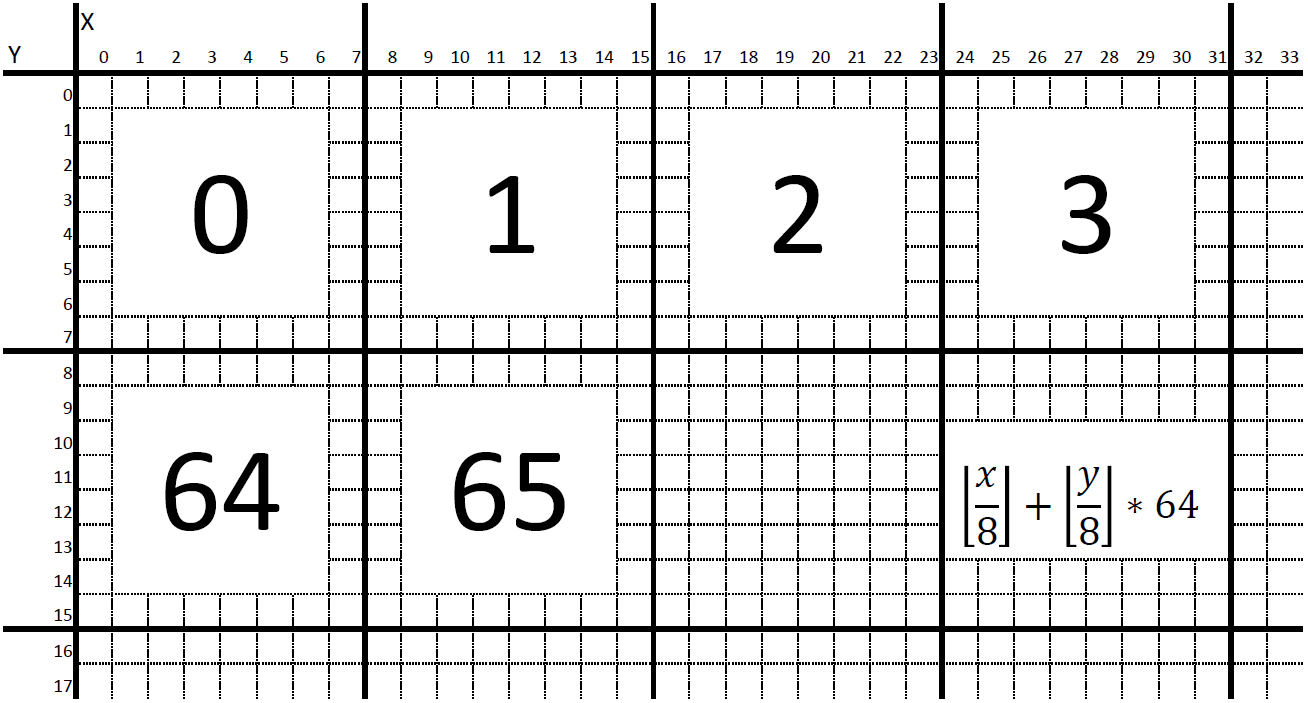
\includegraphics[width=1.0\textwidth]{Bildschirm.png}
	\caption[Veranschaulichung der Adressberechnung der ASCII-Unit]{Veranschaulichung der Adressberechnung anhand des Pixelfelds des Monitors: Links oben wird von 0 ab nach rechts zeilenweise hochgez\"ahlt. Die Adresse des Zeichenfeldes zu dem ein Pixel mit Position (x,y) geh\"ort wird wie folgt berechnet: $\lfloor \frac{x}{8} \rfloor + \lfloor \frac{y}{8} \rfloor * 64$. Aus dem 64-Bit-Vektor berechnet man das Bit f\"ur das aktuelle Pixel so: $(x\:  mod\:  8) + (y\:  mod\:  8) * 8$.}
\end{figure}

Da eine Darstellung von Kleinbuchstaben auf einem 6*6 Bitfeld kaum sinnvoll zu realisieren ist, eine Unterscheidung ohnehin schwierig w\"are und der Fokus nicht auf \"Asthetik lag wurden diese durch Gro{\ss}buchstaben ersetzt.
Nicht zeichenbare ASCII-Zeichen (Zeilenumbr\"uche, Tabulator etc.) werden als leere Zeichen dargestellt, sodass bei der Berechnung der Adresse nicht auf vorangegangene Sonderzeichen geachtet werden muss, was die Implementierung erleichtert. Dadurch muss allerdings die Software die Verwaltung des CHARRAMs \"ubernehmen, um diese Zeichen korrekt darzustellen.\\
Die ASCII-Unit ist wie die VGA-Unit auf 25 MHz getaktet. Denn die VGA-Unit sendet in jedem ihrer Takte die Informationen zu einem Pixel zum Monitor und die ASCII-Unit berechnet in jedem Takt genau die Information, ob das jeweilige Pixel gesetzt oder frei, sprich Wei{\ss} oder Schwarz sein soll. Die Berechnung des Pixels in der ASCII-Unit erfolgt dabei \"uber mehrere Takte hinweg stufenweise und f\"ur jedes Pixel in jedem Frame neu, sodass gleichzeitig f\"ur verschiedene Pixel in verschiedenen Stufen eine Berechnung stattfindet.



\Section{Interface}
Neben dem bereits erw\"ahnten Takteingang gibt es jeweils einen Eingang f\"ur die x- und y-Koordinate des aktuellen Pixels (bzw. Position des Fadenstrahls) aus der VGA-Unit, welche mit jedem Takt aktualisiert werden und ein Ausgangssignal an die VGA-Einheit, welches angibt, ob das aktuelle Pixel gesetzt werden soll oder nicht.\\ Au{\ss}erdem gibt es zur Kommunikation mit dem CHARRAM in der MMU einen Ausgang, welcher die Adresse des Zeichenplatzes des aktuell zu berechnenden Pixels angibt sowie einen Eingang, der im darauffolgenden Takt die ASCII-Nummer des zugeh\"origen Zeichens erh\"alt.\\
Zur CHARMAP, die als ROM fungieret, wird der Takt durchgeleitet und ebenso die aus dem CHARRAM kommende ASCII-Nummer des aktuellen Zeichens, die hierbei als Adresse fungiert. Aus der CHARMAP kommt im darauffolgendem Takt der oben erw\"ahnte 64-Bit-Vektor der das jeweilige Zeichen repr\"asentiert.

\begin{figure}[H]
	\centering
	\label{fig:interface}
		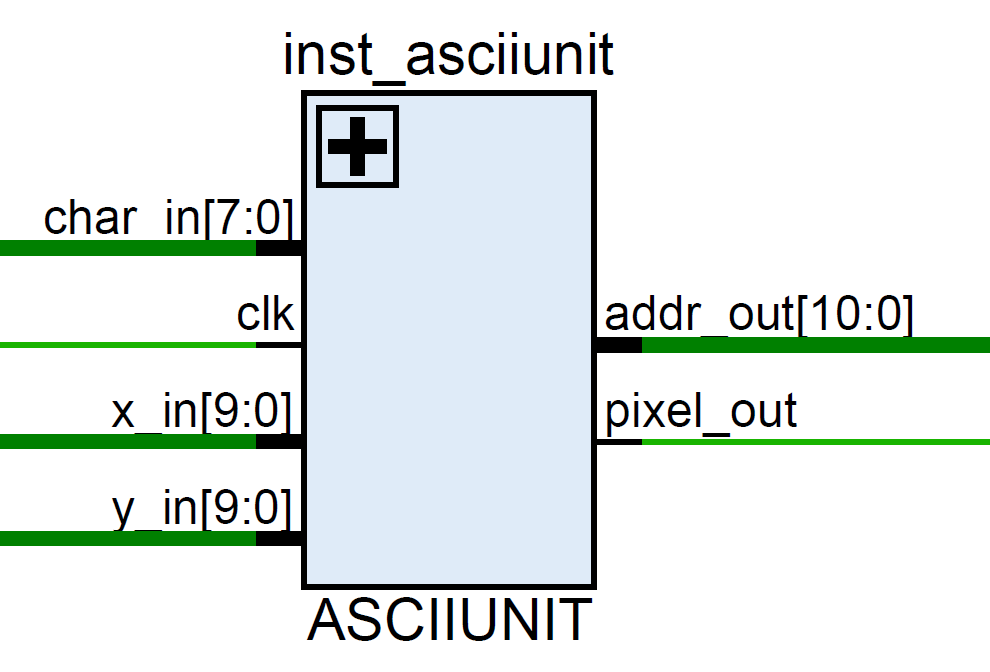
\includegraphics[width=0.3\textwidth]{Asciiunit.png}
	\caption[Interface der ASCII-Unit]{Das Interface der ASCII-Unit}
\end{figure}

\Section{Funktionsweise}
Die stufenweise Berechnung f\"ur jedes Pixel beginnt mit der Verrechnung der x- und y-Koordinate aus der VGA-Einheit. Dazu wird zuerst die x-Koordinate um 2 erh\"oht und in ein internes Signal gespeichert, sodass quasi im Vorraus berechnet wird, ob ein Pixel gesetzt werden wird oder nicht.\\
Im n\"achsten Takt wird daraus die Adresse des aktuellen Zeichen-Platzes berechnet, welche dann durch die MMU in den CHARRAM geleitet wird.\\
Von dort wird im anschlie\ss{}enden Takt die ASCII-Nummer des aktuellen Zeichens geliefert, welche direkt in die CHARMAP weitergeleitet wird. Dies ist auch problemlos bei gleichzeitigem Zugriff der MMU auf den CHARRAM m\"oglich, da dieser als Dual-Port-Blockram realisiert wird. Auch die schnellere Taktung der MMU stellt keine Herausforderung dar: Der jeweilige Lesezugriff erfolgt einfach mehrmals hintereinander. Lediglich falls zwischen den insgesamt 64 Zugriffen pro Frame der ASCII-Unit auf eine Adresse im CHARRAM eben diese Zelle von der MMU \"uberschrieben wird kann es zu einer kurzzeitigen St\"orung kommen: Dieses Zeichen w\"urde dann m\"oglicherweise in diesem Frame falsch dargestellt, was sich im Betrieb allerdings kaum bemerkbar macht.\\
Die CHARMAP liefert im folgenden Takt wiederum den aktuellen 64-Bitvektor aus dem mittels der aktuellen x- und y-Koordinate berechnet wird, ob das Pixel zu setzen ist oder nicht.\\
Diese Information wird dann im letzten Takt an die VGA-Unit zurückgesandt.
\begin{figure}[H]
	\centering
	\label{fig:overview}
		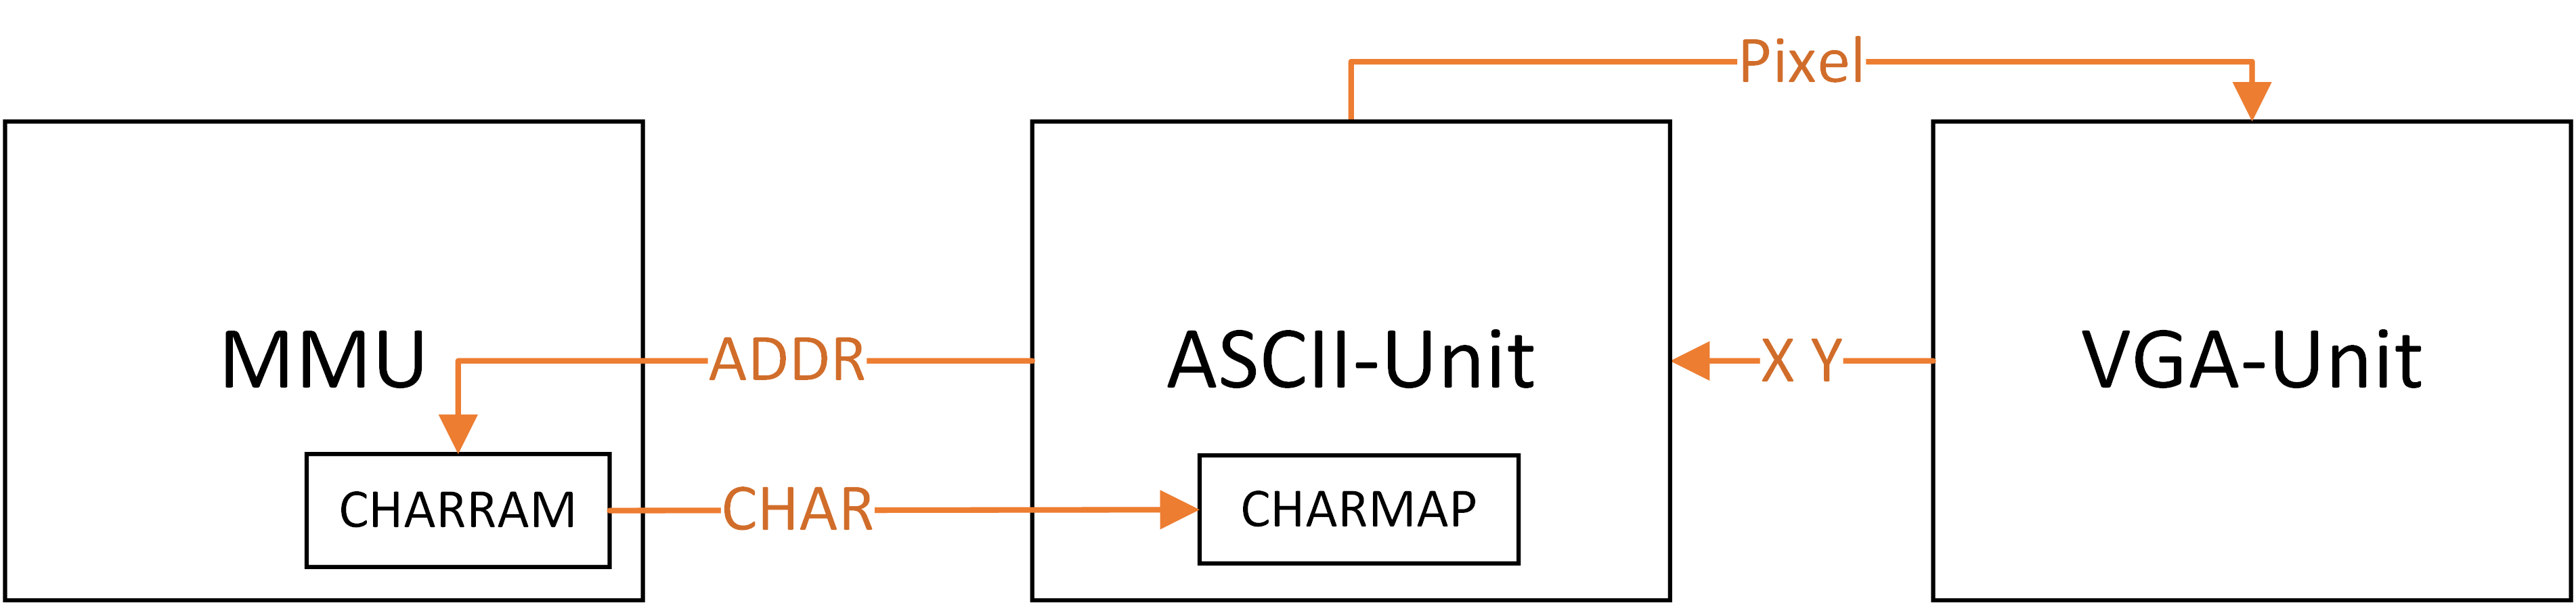
\includegraphics[width=1.0\textwidth]{ASCII.png}
	\caption[\"Ubersicht \"uber die ASCII-Unit]{\"Ubersicht: Beginn bei x- bzw. y-Koordinate; Verrechnung dieser zur Adresse f\"ur CHARRAM; dann Durchleiten in CHARMAP; anschlie\ss{}end Berechnung des Pixels; letztendlich Zur\"ucksenden an VGA-Unit}
\end{figure}

